\chapter{データベース/ネットワーク設計}
\section*{データベース設計}
本システムで用いるDBのER図(p.\pageref{fig:ER図}),テーブル構成図(p.\pageref{tableDesgin1},p.\pageref{tableDesgin2})は記載のとおりである.
\section*{ネットワーク設計}
\figref{fig:ネットワーク設計}は本サービスのネットワーク構成を示す.AWSを用いてネットワークを設計する.構成としてWebサーバ,DB(楽譜,ユーザ)を使用する.
\begin{figure}[b]
    \centering
    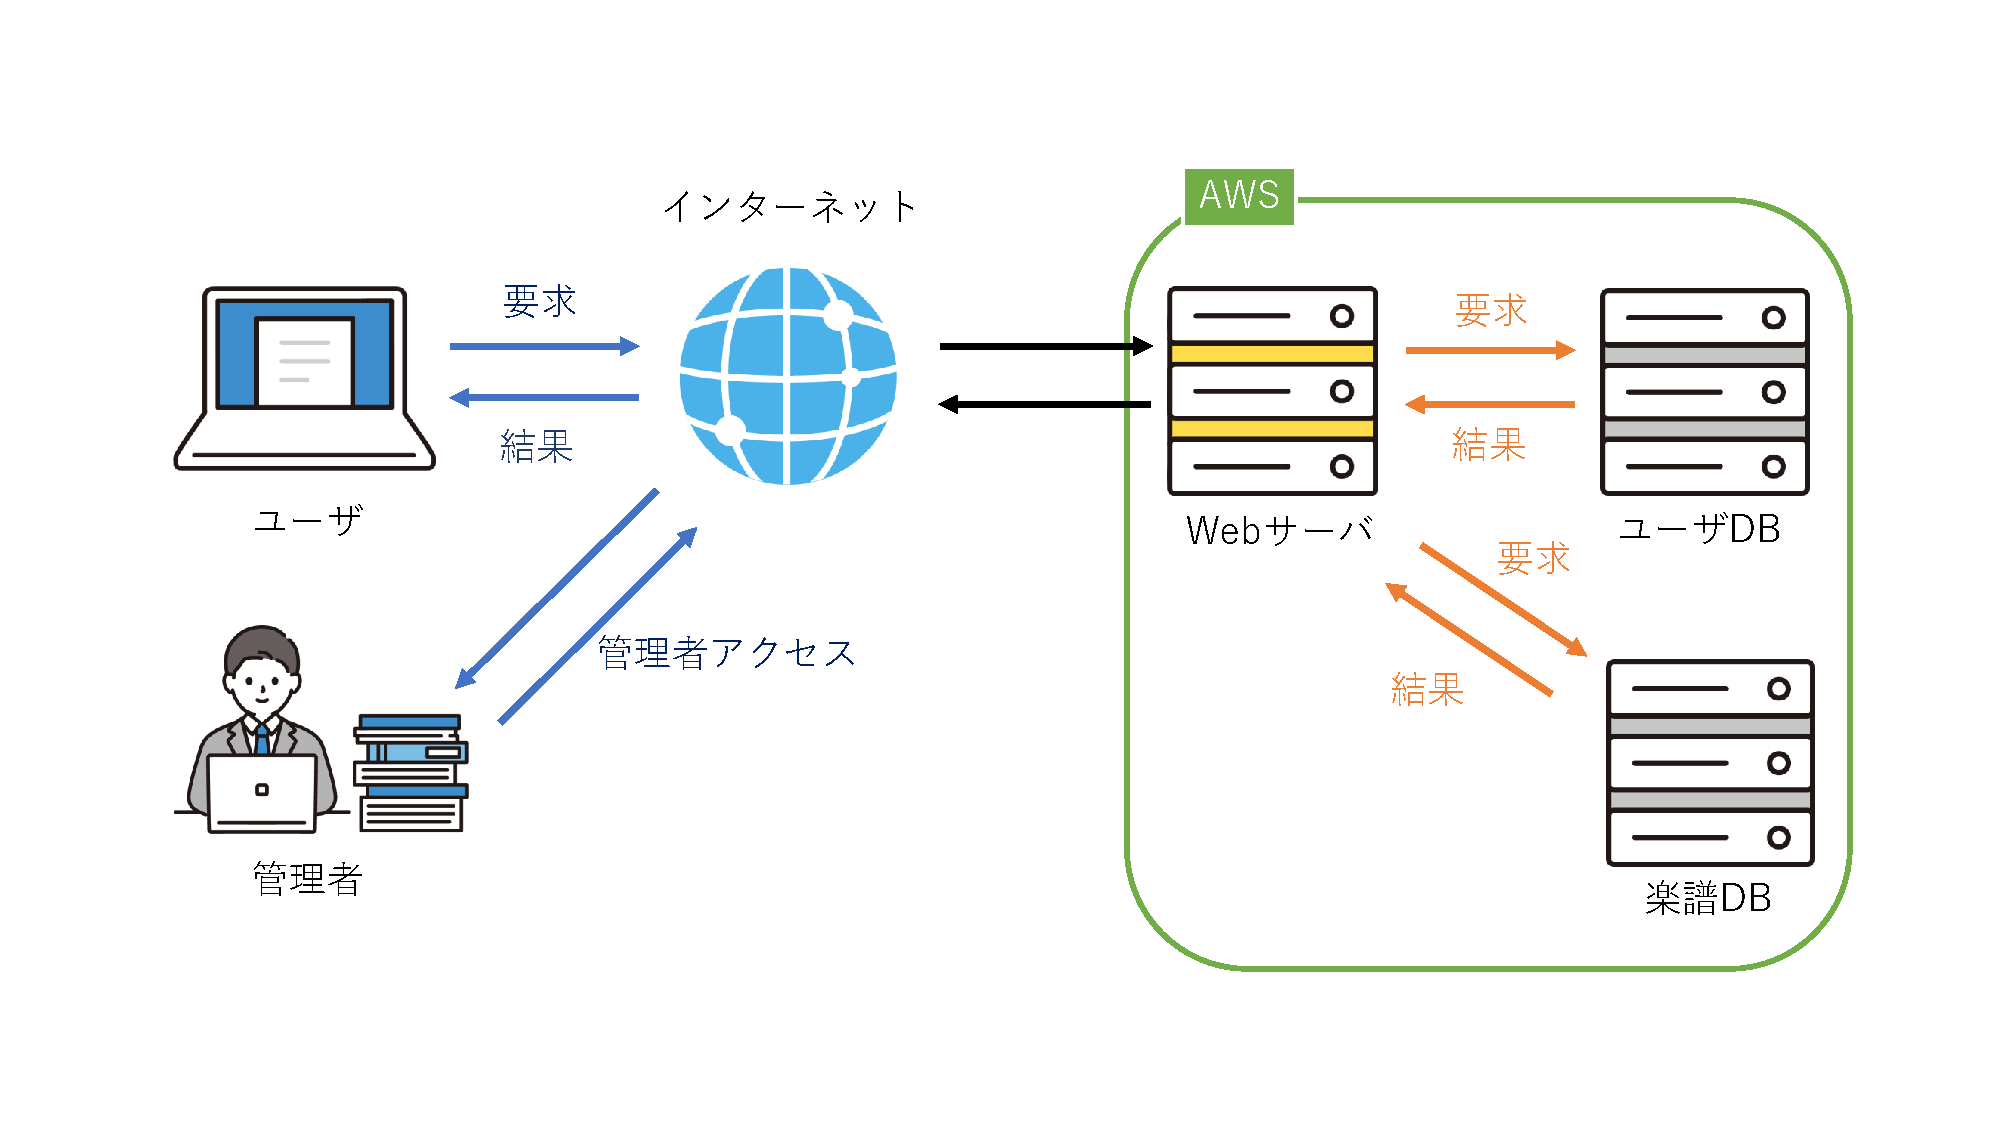
\includegraphics[keepaspectratio,width=\textwidth]{db-nwDesign/networkDesign.pdf}
    \caption{ネットワーク設計}\label{fig:ネットワーク設計}
\end{figure}
\begin{figure}[p]
    \centering
    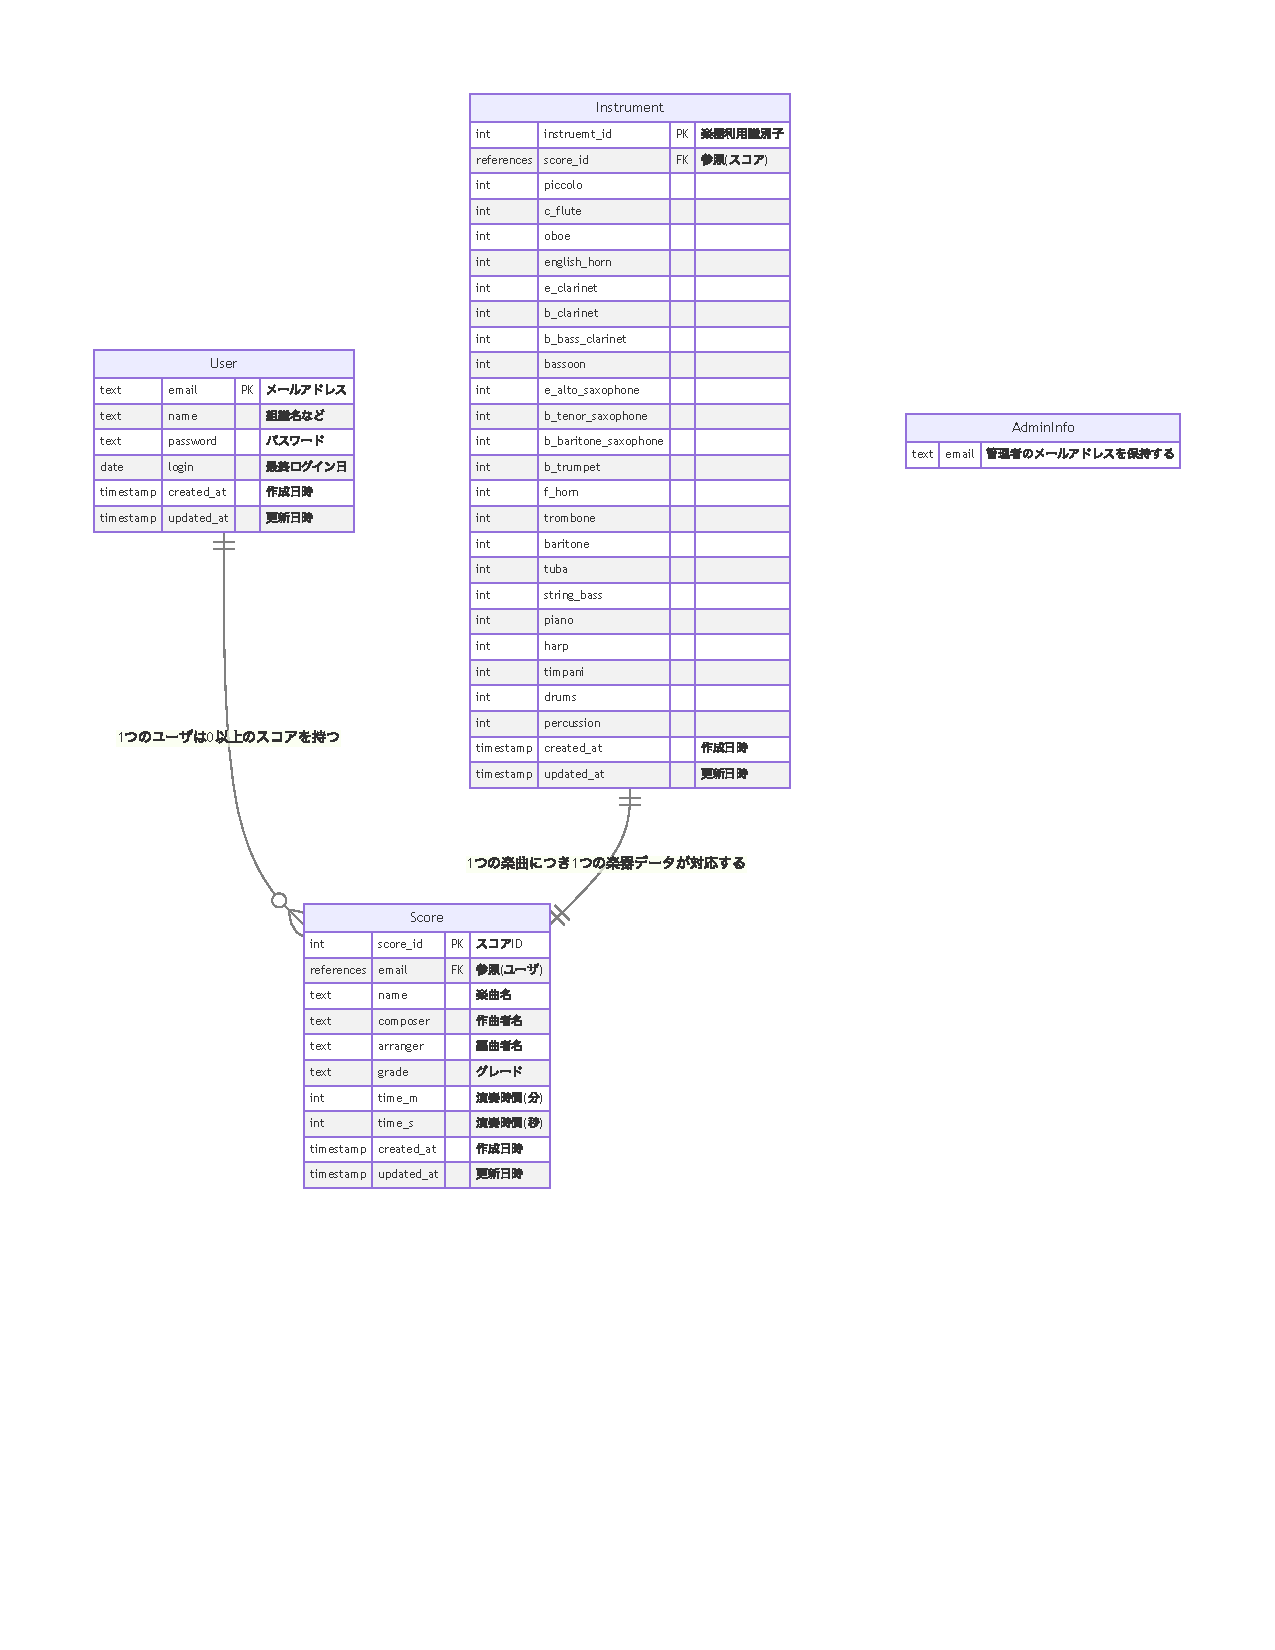
\includegraphics[keepaspectratio,height=.9\textheight]{db-nwDesign/er.pdf}
    \caption{ER図}
    \label{fig:ER図}
\end{figure}
\begin{table}[p]
    \centering
    \caption{データベース名:User}
    \begin{tabularx}{\textwidth}{llcR}
        \hline
        DataName      & DataType    & NOT NULL & Notes                     \\
        \hline
        email         & text        & O        & \texttt{user@example.com} \\
        name          & text        & O        & XX学校吹奏楽部                  \\
        password      & text        & O        & 6文字以上20文字以下の英数字           \\
        login         & date        &          &                           \\
        {{timestamp}} & created\_at & O        & 作成日時(Rails)               \\
        {{timestamp}} & updated\_at & O        & 更新日時(Rails)               \\
        \hline
    \end{tabularx}\\
    \vfill
    \caption{データベース名:Socre}
    \begin{tabularx}{\textwidth}{llcR}
        \hline
        DataName      & DataType    & NOT NULL & Notes       \\
        \hline
        socre\_id     & int         & O        & スコアID       \\
        email         & references  & O        & userの主キーを参照 \\
        name          & text        & O        & 楽曲名         \\
        {{composer}}  & text        &          & 作曲者名        \\
        arranger      & text        &          & 編曲者名        \\
        grade         & text        &          & 難易度         \\
        time\_m       & int         &          & 演奏時間(分)     \\
        time\_s       & int         &          & 演奏時間(秒)     \\
        {{timestamp}} & created\_at & O        & 作成日時(Rails) \\
        {{timestamp}} & updated\_at & O        & 更新日時(Rails) \\
        \hline
    \end{tabularx}
    \label{tableDesgin1}
\end{table}
\begin{table}[p]
    \caption{データベース名:Instrument}
    \begin{tabularx}{\textwidth}{llcR}
        \hline
        DataName               & DataType    & NOT NULL & Notes        \\
        \hline
        instrument\_id         & int         & O        & 主キー          \\
        socre\_id              & references  & O        & score\_idを参照 \\
        piccolo                & int         &          &              \\
        c\_fulute              & int         &          &              \\
        oboe                   & int         &          &              \\
        english\_horn          & int         &          &              \\
        b\_clarinet            & int         &          &              \\
        b\_bass\_clarinet      & int         &          &              \\
        bassoon                & int         &          &              \\
        e\_alto\_saxophone     & int         &          &              \\
        b\_tenor\_saxophone    & int         &          &              \\
        b\_baritone\_saxophone & int         &          &              \\
        b\_trumpet             & int         &          &              \\
        f\_horn                & int         &          &              \\
        trombone               & int         &          &              \\
        baritone               & int         &          &              \\
        baritone\_treble\_clef & int         &          &              \\
        tuba                   & int         &          &              \\
        string\_bass           & int         &          &              \\
        piano                  & int         &          &              \\
        harp                   & int         &          &              \\
        timpani                & int         &          &              \\
        drums                  & int         &          &              \\
        percussion             & int         &          &              \\
        {{timestamp}}          & created\_at & O        & 作成日時(Rails)  \\
        {{timestamp}}          & updated\_at & O        & 更新日時(Rails)  \\
        \hline
    \end{tabularx}
    \label{tableDesgin2}
\end{table}